\chapter{Experiments}
To evaluate the performance of different approaches, there are three experiments:
the maximization extended probability of detection problem, the search problem, and Tuning $\alpha$ parameters.
The EX$1$ is to evaluate the extended probability of target detection (EPD) of different offline approaches with routing constraints in simulations.
The EX$2$ is to evaluate the search time of different approaches with routing constraints in simulations and real world.
%The EX$3$ is to evaluate the search time of changing the parameter $\alpha$ in CBST {\color{olive}to verify wether the $\alpha$ changing will influence results}.
The purpose of EX3 is to evaluate the influence of changing $\alpha$ for search results.

\section{Experiment setup}
In the EX$1$ and EX$2$, there are two different size maps.
The size of  map 1 and map 2 are  $4 \times 4 \times 3$ $(m^3)$ and $8 \times 8 \times 3$ $(m^3)$, respectively.
As shown in Fig.~\ref{fig:Ground_set}, the ground set $S$ is generated with $||S|| = 58.$
The numbers of subgoals in low altitude is more than that in high altitude, due to the camera field of view (FOV).
The index $1$ is start point.
The experimental setup (e.g., camera and drone parameters) is as shown in Table~\ref{tab:drone_info}.
%The minimum altitude, the maximum altitude and the distance between altitude levels are $0.5,$ $3.0$ and $0.3$, respectively.

%The index $1$ in Fig.~\ref{fig:Ground_set} is the start point.
%The minimum altitude in Fig.~\ref{fig:Ground_set} is $0.5;$ the maximum altitude in Fig.~\ref{fig:Ground_set} is $3.0.$
%The distance between altitude levels on the subgoals is $0.3.$
The cost constraints are $10$ and $40,$ respectively.
The cost function $c$ is measured by Euclidean distance.
Note that, since computing routing cost is NP-hard problem, $c$ is approximated by $\hat{c}$ via Nearest Neighbor (NN) algorithm~\cite{rosenkrantz1977analysis} which provides a $\frac{3}{2}-$approximation factor.
%The experimental parameters are at Table.~\ref{tab:cam_info}.
%The range of downward camera is $3.0 (m).$ {\color{olive}Its} horizontal FOV is $60^{\circ}$;
%{\color{olive}its} vertical FOV is $45^{\circ}.$
%{\color{olive}Its} frame rate per second is $10.$
%It represents the camera takes $10$ frames per second.



\begin{table}[htbp]
   \caption{Drone hardware setup in simulation.}
   \begin{center}
     \begin{tabular}{|| c | l | l ||}
     \hline
     Parameter & description & value\\ [0.5ex]
     \hline\hline
     $c_r$ & range & $3.0$ (m) \\
     \hline
     $FOV_h$ & horizontal FOV & $60^{\circ}$ \\
     \hline
     $FOV_v$ & vertical FOV & $45^{\circ}$ \\
     \hline
     $c_{fr}$ & frame rate & $10$ (FPS) \\
     \hline\hline
     $h_{max}$ & flight minimum altitude & $0.5$ (m) \\
     \hline
     $h_{min}$ & flight maximum altitude & $3.0$ (m) \\
     \hline
     $h_{level}$ & flight altitude levels & $0.3$ (m) \\
     \hline
     $\omega_{max}$ & limitation of angular velocity & $42$ (deg/s) \\
     \hline
     $v_{max}$ & limitation of linear velocity & $1$ (m/s) \\
     \hline
    \end{tabular}
   \end{center}
   \label{tab:drone_info}
\end{table}

The target locates in $121$ places uniformly. The drone searches $5$ times in each place.
Hence, there are $605$ times.
The search processing is as follows: The agent takes off and moves to the next subgoal.
If the drone cannot find the target ($P(Z=1) \le 95 \%$), the agent will go through the next path (point) until finding the target ($P(Z=1)\ge 95 \%$) or utilizing all budgets.

There are two setups in the search experiments.
One is offline, the other one is online.
The online approach for the drone is to computes the information to decide the next subgoal(s);
the offline approach for the drone is to compute all subgoals before taking off.
There are two steps in the offline setup.
First, the path is generated by algorithm subject to budget constraints offline.
Second, the agent flies through the path.
There are three steps in the online setup.
First, the path (or the point) is generated by algorithm online.
Second, the agent flies through the path.
Third, the agent repeats first step via new measurements by second step until the terminal condition.

Along with path, the agent updates the probability of target detection ($Z$) in grid map via Bayesian filter.
There are $20 \times 20$ and $40 \times 40$ grids in map 1 and 2, respectively.
When the probability of the cell in grid map is greater than $95\%$ ($P(Z = 1)\ge 95 \%$), the agent finds the target.
Once the agent finds the target, it will land, and the search time is from taking off to landing.
$E[TTD^+]$ denotes the expected time till positive decisions~\cite{chung2011analysis}.

%{\color{olive}There are two terminal conditions.
%One is the agent finds the target ($P(Z = 1)\ge 95 \%$) subject to the budget constraint, the other one is the agent does not find the target {\color{olive}($P(Z = 1)\le 95 \%$)} until utilizing all budget.
%}

\begin{figure}[htbp]
  \centering
  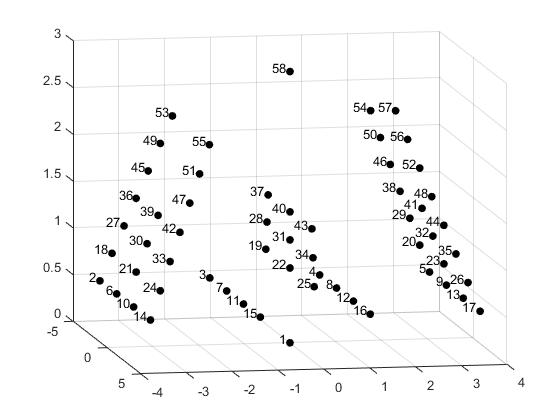
\includegraphics[width=1.0\linewidth]{Ground_set.jpg}
  \caption{Ground set in simulation.}
  \label{fig:Ground_set}
\end{figure}

The map in the real world is a $4\times 4 \times 2 (m^3)$ lobby at the Mathematics department of National Central University (see Fig.~\ref{fig:lobby} (a)).
The target locates in 5 places randomly.
The drone searches 5 times in each place.
Hence, there are 125 times.
The budget $B=10 (m)$ is adopted in this map.
Fig.~\ref{fig:lobby} (a) shows the ground set $|S| = 31$ and the fixed start point is the subgoal $1$.
The target locates in three positions (blue stars) at each search.
%{\color{red} (add 3F experiments!)}
%The drone searches for the target 1 times at each location. %({\color{red}To do (5 times at each location)}).

As shown in Fig.~\ref{fig:nx}, the TD450 is developed by Taiwan Drone 100.
The D435i RGBD camera is to explore the environment while T265 camera is to localize itself.
The YOLOv5~\cite{glenn_jocher_2022_7347926} is adopted to detect objects running on NVIDA Jetson Xavier NX (see Fig.~\ref{fig:lobby} (b)).
The drone's operating system is Ubuntu 18.04 and runs the Robot Operating System (ROS).
The parameters of TD450 hardware setup are shown in Table~\ref{tab:drone_info_nx}.

\begin{table}[htbp]
   \caption{Drone hardware setup in real world.}
   \begin{center}
     \begin{tabular}{|| c | l | l ||}
     \hline
     Parameter & description & value\\ [0.5ex]
     \hline\hline
     $c_r$ & range & $3.0$ (m) \\
     \hline
     $FOV_h$ & horizontal FOV & $69^{\circ}$ \\
     \hline
     $FOV_v$ & vertical FOV & $42^{\circ}$ \\
     \hline
     $c_{fr}$ & frame rate & $30$ (FPS) \\
     \hline\hline
     $h_{max}$ & flight minimum altitude & $1.1$ (m) \\
     \hline
     $h_{min}$ & flight maximum altitude & $2.0$ (m) \\
     \hline
     $h_{level}$ & flight altitude levels & $0.3$ (m) \\
     \hline
     $\omega_{max}$ & limitation of angular velocity & $120$ (deg/s) \\
     \hline
     $v_{max}$ & limitation of linear velocity & $0.2$ (m/s) \\
     \hline
    \end{tabular}
   \end{center}
   \label{tab:drone_info_nx}
\end{table}


\begin{figure}[htbp]
  \centering
  \begin{subfigure}{.4\textwidth}
  \centering
  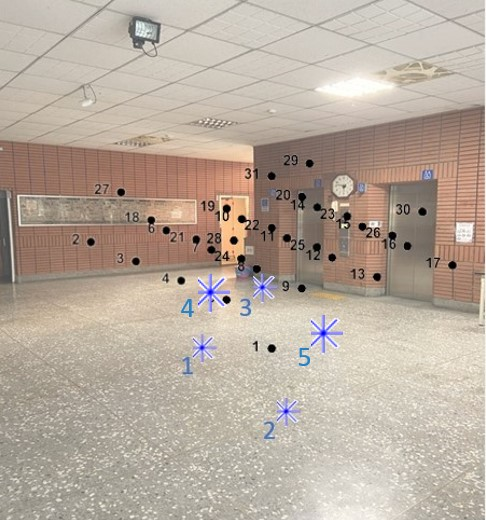
\includegraphics[width=1.0\linewidth]{lobby_and_subgoals.jpg}
  \caption{The lobby environment.}
\end{subfigure}
%\begin{subfigure}{.4\textwidth}
%  \centering
%  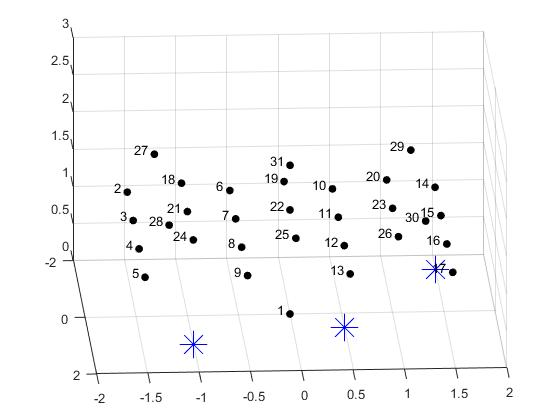
\includegraphics[width=1.0\linewidth]{lobby_sub.jpg}
%  \caption{{\color{olive}Ground set and target locations in real world.}}
%\end{subfigure}
\begin{subfigure}{.4\textwidth}
  \centering
  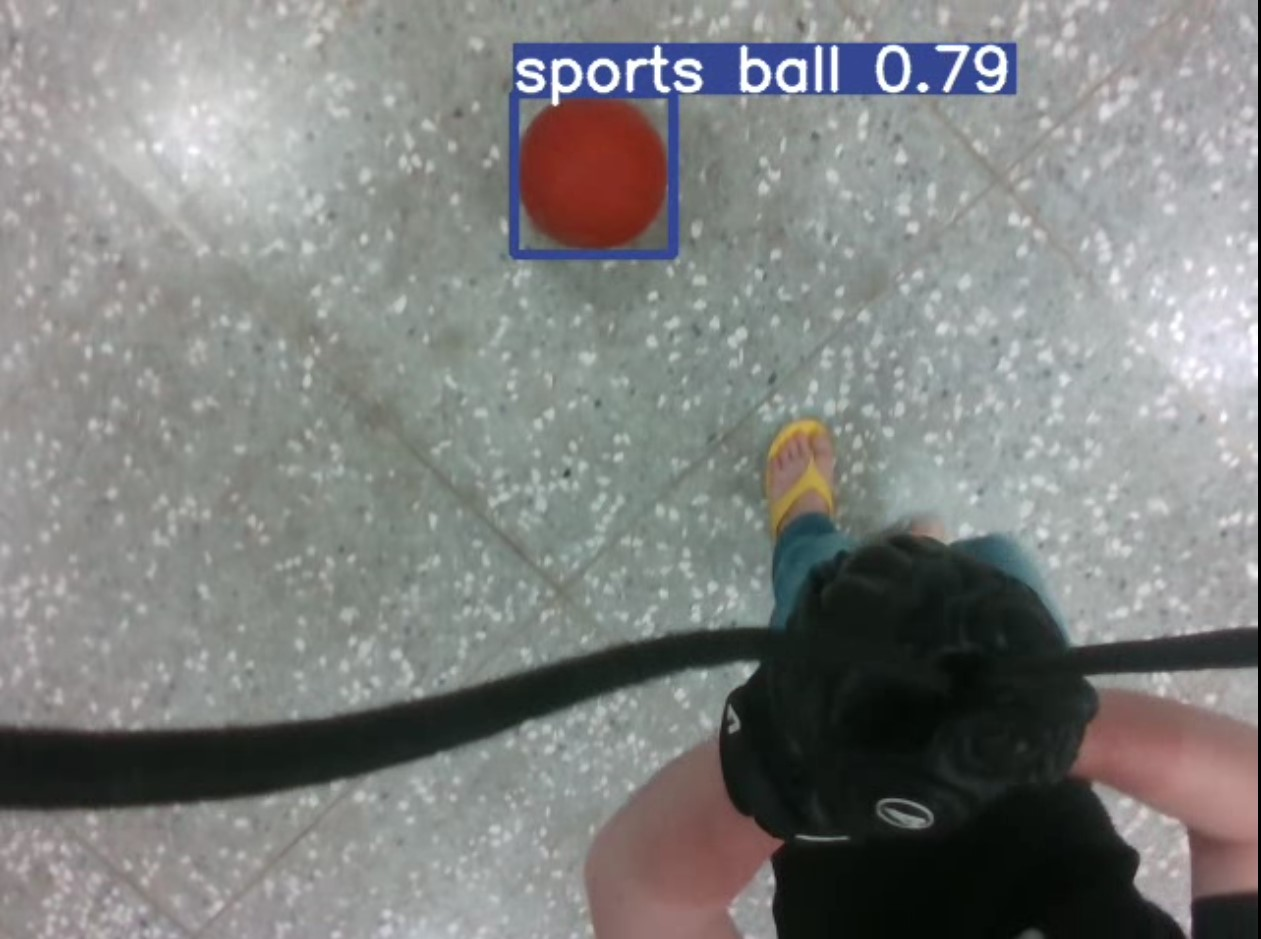
\includegraphics[width=1.0\linewidth]{det.jpg}
  \caption{The detection outcome of YOLOv5.}
\end{subfigure}
  \caption{(a)
  The black points, black decimal numbers,the index 1 in black represent the subgoals, the subgoal indexes and the source node, respectively.
  The blue stars and decimal numbers represent the target locations and the subgoal indexes, respectively.
  (b) The d435i provides the RGB images. The YOLOv5 detects the target in the image. The blue box represents the target location in the image with the detection probability.
  }
  \label{fig:lobby}
\end{figure}

\begin{figure}[htbp]
  \centering
  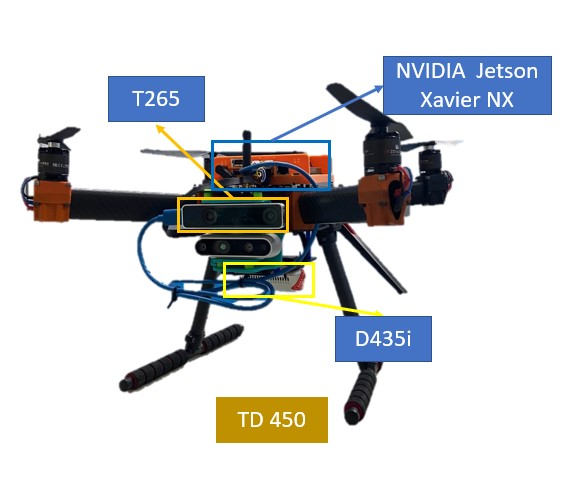
\includegraphics[width=1.0\linewidth]{nx.jpg}
  \caption{The TD450, sensors and development board.}
  \label{fig:nx}
\end{figure}

\section{EX$1$: EPD maximization}


In the experiment, the GCB-CBST is compared with four methods: A-optimality with CMA-ES~\cite{popovic2020informative}, GCB~\cite{zhang2016submodular}, GCB-MST~\cite{lin2023improvement}, and GCB-SPT. CMA-ES is online method, the others are offline methods.


The experiment results in the Gazebo simulation are summarized in Table~\ref{tab:EPD_map}.
Since CMA-ES is online algorithm, the accumulated EPD is not available.
GCB-CBST outperforms other approaches in the accumulated EPD in map 1 and 2.
The tree structures of MST, SPT, and CBST in map 1 and 2 are shown in Fig.~\ref{fig:TSG_map1} and~\ref{fig:TSG_map2}, respectively.
As shown in Fig.~\ref{fig:TSG_map1} (b) and~\ref{fig:TSG_map2} (b),
the tree structure of SPT are inefficient seeing due to the repeated paths.
Since the path in GCB-SPT have high cost-benefit, the accumulated EPD of GCB-SPT is higher than GCB-MST.
%The performance in GCB-CBST is better than that in GCB-MST because the agent will go through the repeated path.
These experiments show that GCB-CBST outperforms the other three methods in the maximal EPD problem.

%The GCB-TSG (MST) is worst case because the agent cannot go through the key point ($v_{58}$ in Fig.~\ref{fig:Ground_set}) that represents the agent will get lots of EPD in this map in Fig.~\ref{fig:TSG_map1}(a),~\ref{fig:TSG_map2}(a).
%As shown in~\ref{fig:TSG_map1}(b),~\ref{fig:TSG_map2}(b), the height of the GCB-TSG (SPT) is $1,$ so the agent will go through the next subgoal and go back to start point recursively. The agent in GCB-TSG (SPT) can go through the key point but wasting resources. The performance in GCB-TSG (SPT) is in median.
%{\color{red} (Read some papers. Check out how to describe the proposed approach is better than others.)}


%\begin{table}[t!]
%   \caption{EPD maximization experiment results in $4\times 4\times 3 (m)$ environment.}
%   \begin{center}
%     \begin{tabular}{| l | l | l | l | l | l |  l | l |} \hline
%     Method & accumulated EPD\\ \hline
%     A-opt with CMA-ES  & NA \\ \hline
%     GCB & $\textbf{0.993}$ \\ \hline
%     GCB-TSG(CBST) & $\textbf{0.958}$ \\ \hline
%     GCB-TSG(MST) & 0.489 \\ \hline
%     GCB-TSG(SPT) & 0.843 \\ \hline
%    \end{tabular}
%   \end{center}
%   \label{tab:EPD_map1}
%\end{table}

\begin{table}[htbp]
   \caption{
   EPD maximization experiment results.
   The accumulated EPD (AEPD) as follows.
   % in $8\times 8\times 3 (m)$ environment.
   }
   \begin{center}
     \begin{tabular}{| c | l | l | l | l | l |  l | l |} \hline
     Method & AEPD (map1) & AEPD (map2)\\ \hline
     A-opt with CMA-ES  & NA & NA \\ \hline
     GCB           & 0.90 & 0.80\\ \hline
     GCB-CBST & $\textbf{0.99}$ & $\textbf{0.84}$ \\ \hline
     GCB-MST  & 0.489 & 0.47 \\ \hline
     GCB-SPT  & 0.843 & 0.52 \\ \hline
%     2 & A-opt with CMA-ES  & NA \\ \hline
%     2 & GCB            & 0.80 \\ \hline
%     2 & GCB-CBST & $\textbf{0.84}$ \\ \hline
%     2 & GCB-MST  & 0.47 \\ \hline
%     2 & GCB-SPT  & 0.52 \\ \hline
    \end{tabular}
   \end{center}
   \label{tab:EPD_map}
\end{table}

\begin{figure}[htbp]
 \begin{center}
\begin{subfigure}{.45\textwidth}
  \centering
  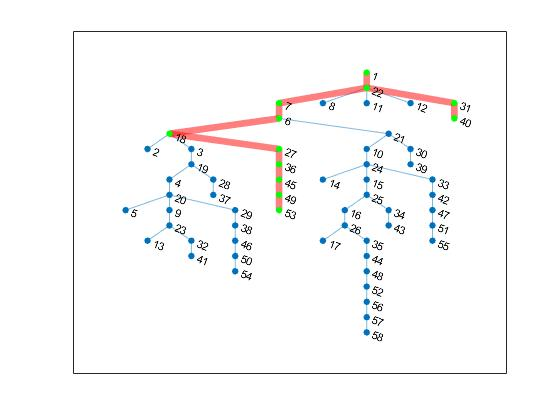
\includegraphics[width=1.0\linewidth]{mst_map1.jpg}
  \caption{The tree structure of MST}
\end{subfigure}
\begin{subfigure}{.45\textwidth}
  \centering
  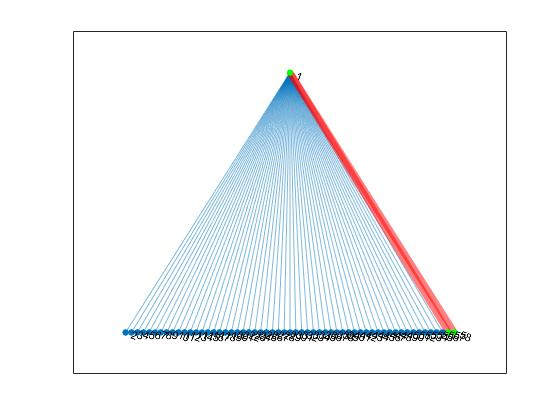
\includegraphics[width=1.0\linewidth]{spt_map1.jpg}
  \caption{The tree structure of SPT}
\end{subfigure}
\begin{subfigure}{.45\textwidth}
  \centering
  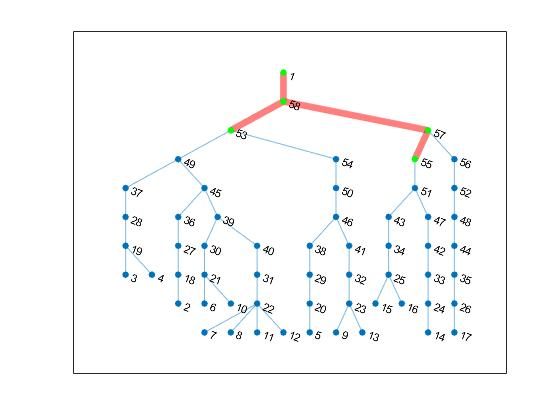
\includegraphics[width=1.0\linewidth]{f_c_map1.jpg}
  \caption{The tree structure of CBST}
\end{subfigure}
\caption{The blue circles represent the ground set, the green circle represent the picked subgoals, and the red lines represent the path, respectively. There are three tree structures in map1.}
\label{fig:TSG_map1}
 \end{center}
 \end{figure}

\begin{figure}[htbp]
 \begin{center}
\begin{subfigure}{.45\textwidth}
  \centering
  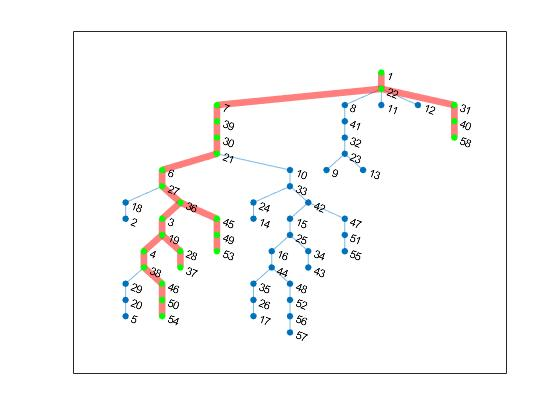
\includegraphics[width=1.0\linewidth]{mst_map2.jpg}
  \caption{The tree structure of MST}
\end{subfigure}
\begin{subfigure}{.45\textwidth}
  \centering
  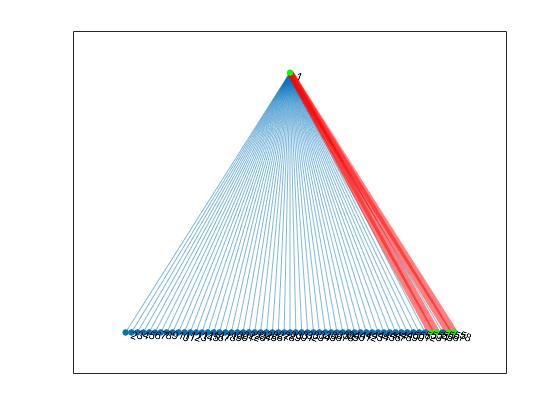
\includegraphics[width=1.0\linewidth]{spt_map2.jpg}
  \caption{The tree structure of SPT}
\end{subfigure}
\begin{subfigure}{.45\textwidth}
  \centering
  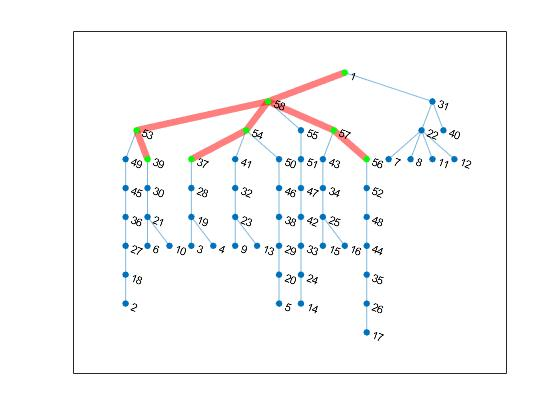
\includegraphics[width=1.0\linewidth]{f_c_map2.jpg}
  \caption{The tree structure of CBST}
\end{subfigure}
\caption{The blue circles represent the ground set, the green circle represent the picked subgoals, and the red lines represent the path, respectively. There are three tree structures in map2.}
\label{fig:TSG_map2}
 \end{center}
 \end{figure}


\section{EX$2$: Search experiment}

The goal of the drone is to find the target as soon as possible subject to budget constraint, so the metrics in this experiment are expected time till positive decisions ($\mathbb{E}$[TTD$^+$]) and success rate.

The parameters are same as EX$1$.

\subsection{Simulation}
To evaluate the search performance, the expected time till positive decision ($\mathbb{E}$[TTD$^+$]) is compared (see Fig.~\ref{fig:ETTD_map1} and~\ref{fig:ETTD_map2}).
GCB-CBST outperforms other four methods in $\mathbb{E}$[TTD$^+$].
GCB-CBST and GCB-SPT are competitive in map 1 since the drone moves to high cost-benefit subgoals.
However, the success rate in GCB-SPT is less than that in GCB-CBST since the path in GCB-SPT is inefficient.
% $\cong$ GCB-TSG (SPT) $\le$ GCB $\cong$ A-opt with CMA-ES $\le$ GCB-TSG (SPT);
%accuracy: GCB $\ge$ GCB-TSG (CBST) $\ge$ GCB-TSG (SPT) $\ge$ A-opt with CMA-ES $\ge$ GCB-TSG (MST).
%
%{\color{blue}The E[TTD$^+$] of GCB-CBST and SPT are better than that of GCB.
%The drone moves to the important subgoal at the first step along the paths obtained by the GCB-CBST and the GCB-SPT.
%Hence, the drone finds the target quickly.
%}


The success rates of the GCB and GCB-CBST are competitive in map 2 (see Table~\ref{tab:ETTD_map}).
The success rate of the GCB is higher than that of the GCB-CBST in map 1 (see Table~\ref{tab:ETTD_map}).
In the GCB-CBST path, the drone moves to the repeated subgoals. Hence, it has fewer false detections than GCB does.
GCB-CBST attains the a little less success rate than GCB in map1 because the drone moves to the repeated subgoals in GCB-CBST.

%The GCB-TSG (MST) is the worst case in E[TTD$^+$] and accuracy.
%The GCB-TSG (CBST) and GCB-TSG (SPT) outperform other three method in E[TTD$^+$].
%However, the path in GCB-TSG (SPT) is short, the accuracy in GCB-TSG (SPT) is worse than GCB-TSG (CBST) and GCB. The GCB is better than GCB-TSG (CBST) in accuracy.
In summary, GCB-CBST is the best method for search tasks, since it can move through the high cost-benefit subgoals immediately and repeatedly.


%{\color{olive}As shown in Table~\ref{tab:ETTD_map2}, the results are similar to Table.~\ref{tab:ETTD_map1}. The difference lies in the fact that previously important points have become relatively less important, resulting in poorer performance of GCB-TSG (SPT).
%On the other hand, GCB-TSG (CBST) still outperforms GCB in terms of E[TTD$^+$].
%}

\begin{table}[htbp]
   \caption{Search experiment results reveal indicators success rate and $\mathbb{E}$[TTD$^+$] in map1 and map2. }
   \begin{center}
     \begin{tabular}{| c | l | l | l | l | l |  l | l |} \hline
      \multirow{2}{*}{Method} & \multicolumn{2}{c|}{Map1} & \multicolumn{2}{c|}{Map2}\\ \cline{2-5}
        & $\mathbb{E}$[TTD$^+$] & success rate & $\mathbb{E}$[TTD$^+$] & success rate\\ \hline\hline
       CMA-ES  & 12.6  & 0.77& 85.7  & 0.28\\ \hline
      GCB & 12.6  & $\textbf{0.96}$ & 30.4  & $\textbf{0.73}$ \\ \hline
      GCB-CBST & $\textbf{5.9}$  & 0.8& $\textbf{26.9}$  & 0.705\\ \hline
      GCB-MST & 18.4 & 0.44  & 48.3 & 0.30 \\ \hline
      GCB-SPT & 6.0 & 0.75 & 30.5 & 0.43\\ \hline
%     2 & A-opt with CMA-ES  & 85.7  & 0.28\\ \hline
%     2 & GCB & 30.4  & $\textbf{0.73}$ \\ \hline
%     2 & GCB-CBST & $\textbf{26.9}$  & 0.70\\ \hline
%     2 & GCB-MST & 48.3 & 0.30 \\ \hline
%     2 & GCB-SPT & 30.5 & 0.43 \\ \hline
    \end{tabular}
   \end{center}
   \label{tab:ETTD_map}
\end{table}

\begin{figure}[htbp]
 \begin{center}
\begin{subfigure}{.30\textwidth}
  \centering
  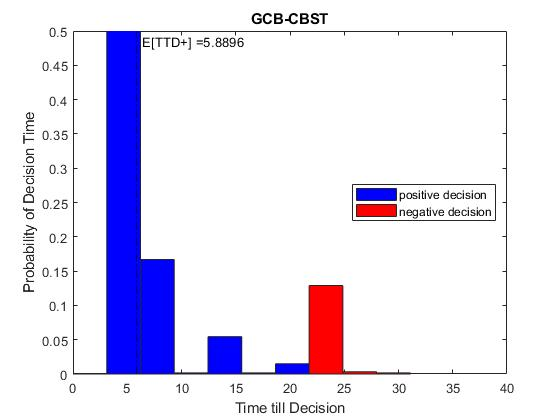
\includegraphics[width=1.0\linewidth]{GCB_CBST_ETTD_map1.jpg}
  \caption{$\mathbb{E}[TTD]$ of GCB-CBST}
\end{subfigure}
\begin{subfigure}{.30\textwidth}
  \centering
  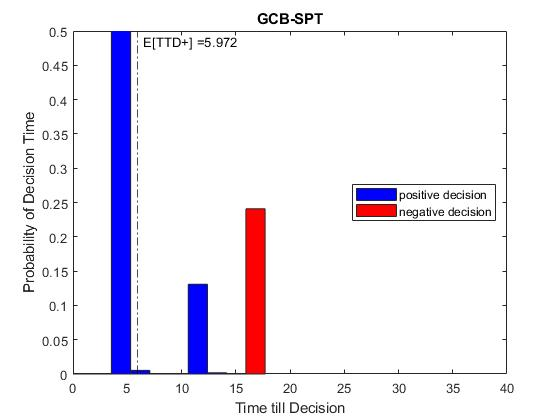
\includegraphics[width=1.0\linewidth]{GCB_SPT_ETTD_map1.jpg}
  \caption{$\mathbb{E}[TTD]$ of GCB-SPT}
\end{subfigure}
\begin{subfigure}{.30\textwidth}
  \centering
  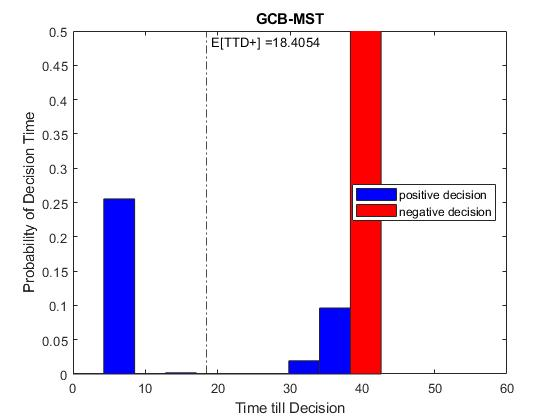
\includegraphics[width=1.0\linewidth]{GCB_MST_ETTD_map1.jpg}
  \caption{$\mathbb{E}[TTD]$ of GCB-MST}
\end{subfigure}
\begin{subfigure}{.30\textwidth}
  \centering
  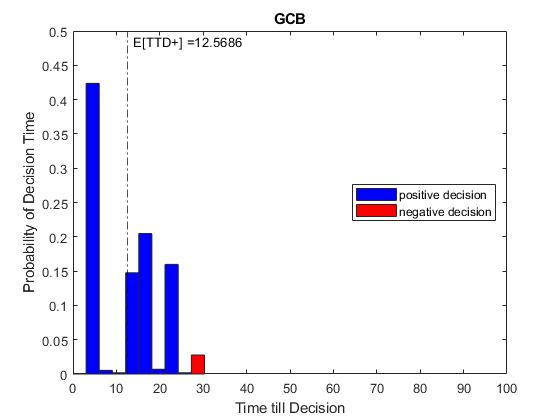
\includegraphics[width=1.0\linewidth]{GCB_ETTD_map1.jpg}
  \caption{$\mathbb{E}[TTD]$ of GCB}
\end{subfigure}
\begin{subfigure}{.30\textwidth}
  \centering
  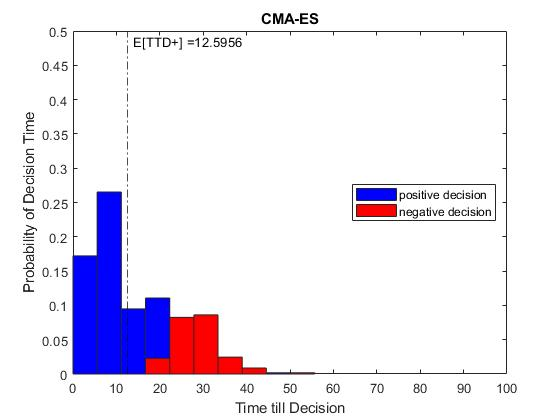
\includegraphics[width=1.0\linewidth]{A_ETTD_map1.jpg}
  \caption{$\mathbb{E}[TTD]$ of CMA-ES}
\end{subfigure}
\caption{$\mathbb{E}[TTD]$ of different tree-structured cost in map1. The x-axis and y-axis represent time (s) and probability, respectively.}
\label{fig:ETTD_map1}
 \end{center}
 \end{figure}

\begin{figure}[htbp]
 \begin{center}
\begin{subfigure}{.30\textwidth}
  \centering
  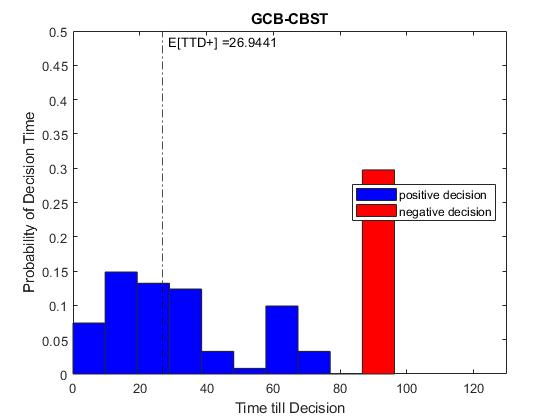
\includegraphics[width=1.0\linewidth]{GCB_CBST_ETTD_map2.jpg}
  \caption{$\mathbb{E}[TTD]$ of GCB-CBST}
\end{subfigure}
\begin{subfigure}{.30\textwidth}
  \centering
  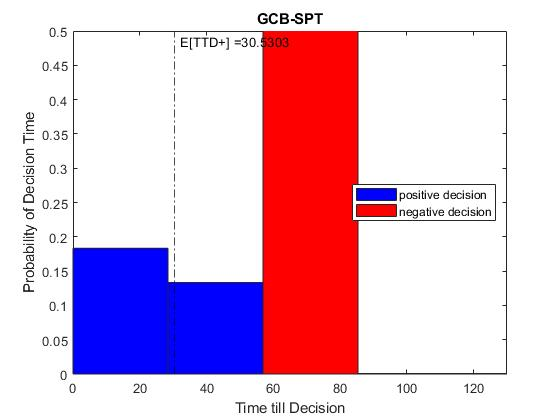
\includegraphics[width=1.0\linewidth]{GCB_SPT_ETTD_map2.jpg}
  \caption{$\mathbb{E}[TTD]$ of GCB-SPT}
\end{subfigure}
\begin{subfigure}{.30\textwidth}
  \centering
  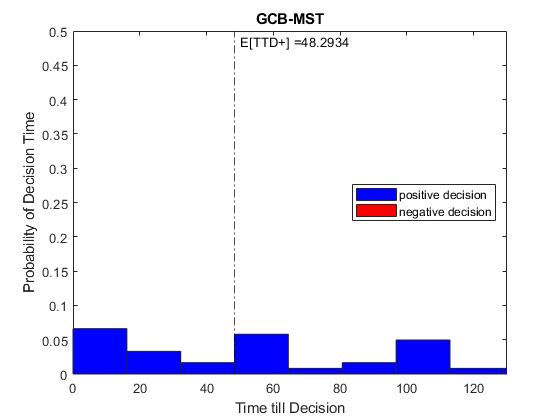
\includegraphics[width=1.0\linewidth]{GCB_MST_ETTD_map2.jpg}
  \caption{$\mathbb{E}[TTD]$ of GCB-MST}
\end{subfigure}
\begin{subfigure}{.30\textwidth}
  \centering
  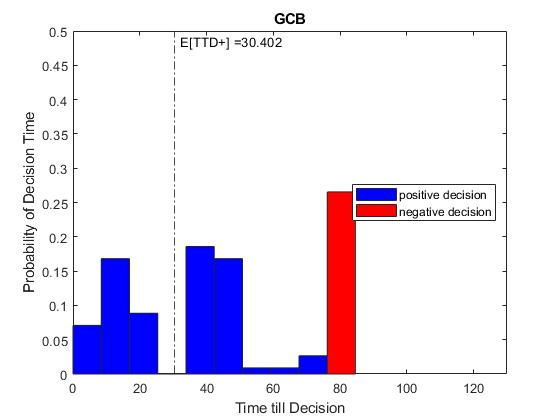
\includegraphics[width=1.0\linewidth]{GCB_ETTD_map2.jpg}
  \caption{$\mathbb{E}[TTD]$ of GCB}
\end{subfigure}
\begin{subfigure}{.30\textwidth}
  \centering
  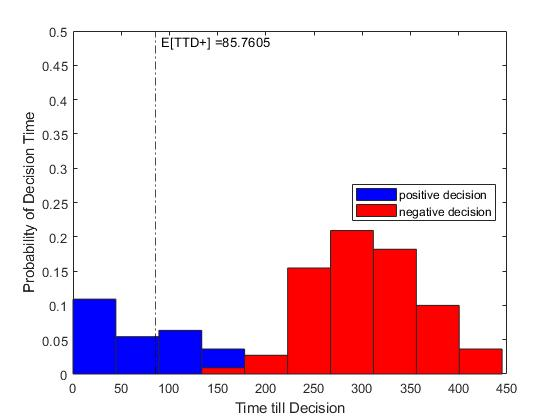
\includegraphics[width=1.0\linewidth]{A_ETTD_map2.jpg}
  \caption{$\mathbb{E}[TTD]$ of CMA-ES}
\end{subfigure}
\caption{$\mathbb{E}[TTD]$ of different tree-structured cost in map2. The x-axis and y-axis represent time (s) and probability, respectively.}
\label{fig:ETTD_map2}
 \end{center}
 \end{figure}
\clearpage
\subsection{Real world}
The tree structures of GCB-CBST, GCB-MST, and GCB-SPT are shown in Fig.~\ref{fig:TSG_lobby}.
GCB-CBST outperforms the other four methods in $\mathbb{E}$[TTD$^+$] (see Table~\ref{tab:ETTD_lobby}).
The height in real world is lower than that in the simulation,
so the path in GCB-SPT does not have high coverage.
The $\mathbb{E}$[TTD$^+$] in GCB-SPT is the worst.

The GCB-CBST outperforms the other four methods in success rate (see Table~\ref{tab:ETTD_lobby}),
since the GCB-CBST must go to subgoals via tree structure, and the drone moves to the repeated subgoals which have high cost-benefit values.
The GCB-MST and GCB-SPT are the worst in success rate.

These experiments show that GCB-CBST outperforms the other four benchmarks in search problems.

\begin{table}[htbp]
   \caption{Search experiment results reveal indicators success rate and $\mathbb{E}$[TTD$^+$] in real world. }
   \begin{center}
     \begin{tabular}{| c | l | l | l | l | l |  l | l |} \hline
      %\multirow{2}{*}{Method} & \multicolumn{2}{c|}{Map1} & \multicolumn{2}{c|}{Map2}\\ \cline{2-5}
        & $\mathbb{E}$[TTD$^+$] & success rate\\ \hline\hline
      CMA-ES  & 86.91 & 0.88\\ \hline
      GCB     & 69.23  & 0.88\\ \hline
      GCB-CBST& $\textbf{51.92}$ & $\textbf{1.00}$\\ \hline
      GCB-MST & 68.77  & 0.52\\ \hline
      GCB-SPT & 79.59  & 0.68\\ \hline
%     2 & A-opt with CMA-ES  & 85.7  & 0.28\\ \hline
%     2 & GCB & 30.4  & $\textbf{0.73}$ \\ \hline
%     2 & GCB-CBST & $\textbf{26.9}$  & 0.70\\ \hline
%     2 & GCB-MST & 48.3 & 0.30 \\ \hline
%     2 & GCB-SPT & 30.5 & 0.43 \\ \hline
    \end{tabular}
   \end{center}
   \label{tab:ETTD_lobby}
\end{table}

\begin{figure}[htbp]
 \begin{center}
\begin{subfigure}{.45\textwidth}
  \centering
  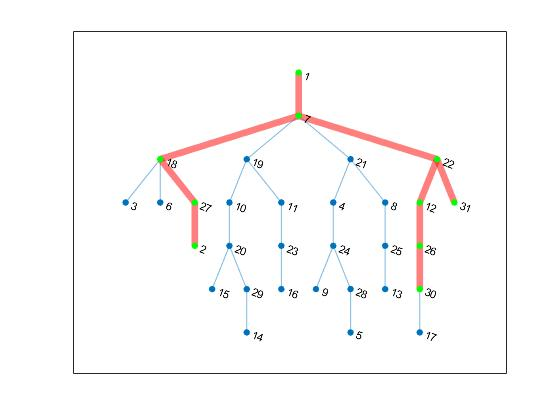
\includegraphics[width=1.0\linewidth]{lobby_mst_10.jpg}
  \caption{The tree structure of MST}
\end{subfigure}
\begin{subfigure}{.45\textwidth}
  \centering
  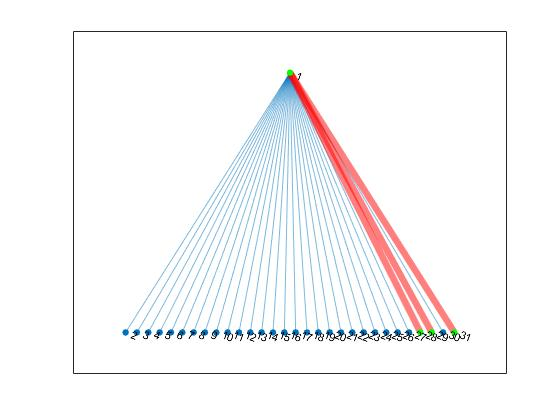
\includegraphics[width=1.0\linewidth]{lobby_spt_10.jpg}
  \caption{The tree structure of SPT}
\end{subfigure}
\begin{subfigure}{.45\textwidth}
  \centering
  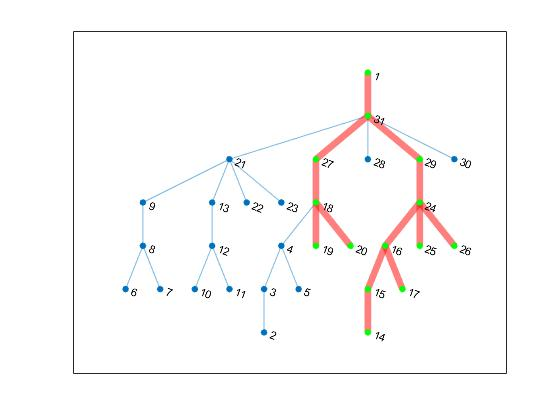
\includegraphics[width=1.0\linewidth]{lobby_cbst_10.jpg}
  \caption{The tree structure of CBST}
\end{subfigure}
\caption{Three tree structures in the lobby environment.
The blue circles and green circles represent the ground set and the picked subgoals, respectively.
The red lines represent the paths. }
\label{fig:TSG_lobby}
 \end{center}
 \end{figure}







%\begin{table}[t!]
%   \caption{Search experiment results in $8\times 8\times 3 (m)$ environment.
%   {\color{red} (merge these two table using map 1 and map 2.)}
%   }
%   \begin{center}
%     \begin{tabular}{| l | l | l | l | l | l |  l | l |} \hline
%     Method & E[TTD$^+$] & Accuracy\\ \hline
%     2 & A-opt with CMA-ES  & 85.7  & 0.28\\ \hline
%     2 & GCB & 30.4  & $\textbf{0.73}$ \\ \hline
%     2 & GCB-TSG(CBST) & $\textbf{29.7}$  & 0.65\\ \hline
%     2 & GCB-TSG(MST) & 33.8 & 0.41 \\ \hline
%     2 & GCB-TSG(SPT) & 33.8 & 0.4 \\ \hline
%    \end{tabular}
%   \end{center}
%   \label{tab:ETTD_map2}
%\end{table}

\section{EX$3$: $\alpha$ tuning}
The $\alpha$ ranges from $0$ to $1$ with an interval of $0.05$.
In the map1, the alpha values generate 4 kinds of tree structures.
the alpha ranges are $0\sim 0.15$, $0.2\sim 0.25$, $0.3\sim 0.4$ and $0.4\sim 1$.
The corresponding sets are $S_0$, $S_1$, $S_2$ and $S_3$ in Fig.~\ref{fig:trees_map1}.
In the map2, the alpha values generate 6 kinds of tree structures.
the alpha ranges are $0$, $0.05$, $0.1\sim 0.15$, $0.2$, $0.25\sim 0.5$ and $0.55\sim 1$.
The corresponding sets are $M_0$, $M_1$, $M_2$, $M_3$, $M_4$ and $M_5$ in Fig.~\ref{fig:trees_map2}.

As shown in Table~\ref{tab:ETTD_alpha_map1}, since map 1 is not big enough, the results in different tree structures in GCB-CBST show insignificant differences.
As shown in Table~\ref{tab:ETTD_alpha_map2}, there are significant difference between $\alpha=0$ and $\alpha=1$ since the map 2 ($8\times8\times3 (m^3)$) is bigger than map 1 ($4\times4\times3 (m^3)$).
The cost function with parameter $\alpha=0$ is the best in $\mathbb{E}$[TTD$^+$], because the tree structure is minimum weight spanning tree.
In the MST algorithm, it is possible to generate edges with the minimum total weight, which results in shorter distances between subgoals.
Consequently, a better $\mathbb{E}$[TTD$^+$] can be achieved.
In the map 2, the $M_3, M_4$ and $M_5$ are inefficient compared to $M_0$, $M_1$ and $M_2$ in Fig.~\ref{fig:trees_map2}.

In summary, the performance when $\alpha$ approaches 0 is better than the performance when $\alpha$ approaches 1
due to the path efficiency.
How to tune an optimal $\alpha$ is still an issue.
The $\alpha=0$ could be a fast solution in search experiments.

%Specifically, when $\alpha$=0, $\mathbb{E}$[TTD$^+$] is optimal due to the presence of minimum weight {\color{red} ???? what do you mean?}.
%However, for $\alpha=0.05$ to $1$, it could achieve better success rate with more traversed nodes.

%In CBST algorithm, the agent can go through the high cost-benefit subgoals immediately in map1, so results in different tree structures in GCB-CBST show insignificant differences.

%{\color{red} (What's the conclusion of EX3? It reflects the purpose or not?) }

\begin{table}[htbp]
   \caption{Search experiment results reveal indicators success rate and $\mathbb{E}$[TTD$^+$] in map 1 with different $\alpha$.}
   \begin{center}
     \begin{tabular}{| c | l | l | l | l | l |  l | l |} \hline
     $\alpha$ & E[TTD$^+$] & Success rate\\ \hline
     $0\sim 0.15$  & $7.85$  & $\textbf{0.74}$\\ \hline
     $0.2\sim 0.25$ & $\textbf{5.76}$  & $0.60$ \\ \hline
     $0.3\sim 0.4$ & $6.48$  & $0.63$\\ \hline
     $0.45\sim 1$ & $6.58$ & $0.64$ \\ \hline
    \end{tabular}
   \end{center}
   \label{tab:ETTD_alpha_map1}
\end{table}

\begin{table}[htbp]
   \caption{Search experiment results reveal indicators success rate and $\mathbb{E}$[TTD$^+$] in map 2 with different $\alpha$.}
   \begin{center}
     \begin{tabular}{| c | l | l | l | l | l |  l | l |} \hline
     $\alpha$ & E[TTD$^+$] & Success rate\\ \hline
     $0$             & $\textbf{26.9}$  & $0.70$\\ \hline
     $0.05$          & $38.8$           & $\textbf{0.83}$\\ \hline
     $0.1\sim 0.15$  & $38.5$           & $\textbf{0.83}$\\ \hline
     $0.2$           & $34.1$           & $0.62$ \\ \hline
     $0.25\sim 0.5$  & $38$             & $0.50$\\ \hline
     $0.55\sim 1$    & $30.5$           & $0.43$ \\ \hline
    \end{tabular}
   \end{center}
   \label{tab:ETTD_alpha_map2}
\end{table}

\begin{figure}[htbp]
 \begin{center}
\begin{subfigure}{.45\textwidth}
  \centering
  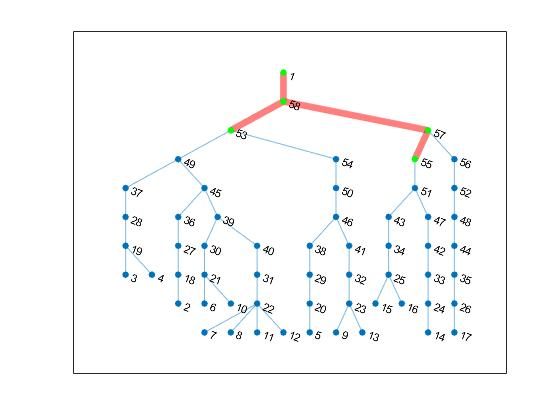
\includegraphics[width=1.0\linewidth]{alpha0.jpg}
  \caption{The tree structure of $S_0$}
\end{subfigure}
\begin{subfigure}{.45\textwidth}
  \centering
  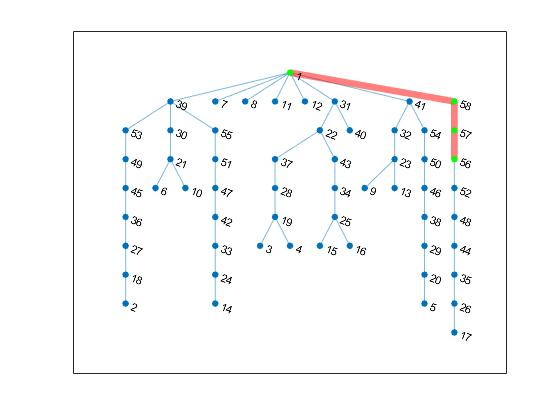
\includegraphics[width=1.0\linewidth]{alpha1.jpg}
  \caption{The tree structure of $S_1$}
\end{subfigure}
\begin{subfigure}{.45\textwidth}
  \centering
  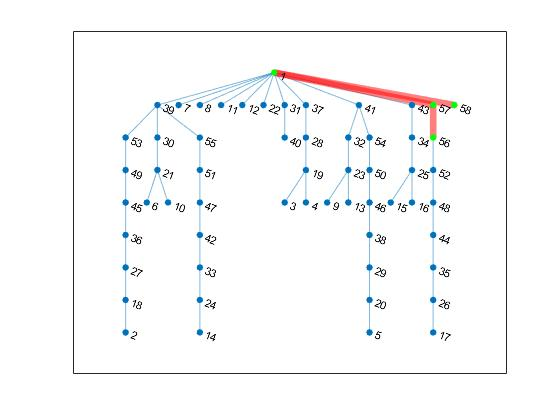
\includegraphics[width=1.0\linewidth]{alpha2.jpg}
  \caption{The tree structure of $S_2$}
\end{subfigure}
%\caption{The blue circles represent the ground set, the green circle represent the picked subgoals, and the red lines represent the path, respectively. There are three tree structures in map 1.}
%\end{center}
%\end{figure}
%
%\begin{figure}[htbp]
%\ContinuedFloat
%\begin{center}
\begin{subfigure}{.45\textwidth}
  \centering
  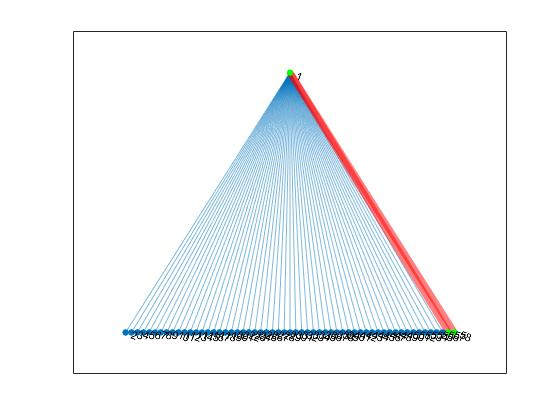
\includegraphics[width=1.0\linewidth]{alpha3.jpg}
  \caption{The tree structure of $S_3$}
\end{subfigure}
\caption{The blue circles represent the ground set, the green circle represent the picked subgoals, and the red lines represent the path, respectively. There are three tree structures in map 1.}
\label{fig:trees_map1}
 \end{center}
 \end{figure}

\begin{figure}[htbp]
 \begin{center}
 \begin{subfigure}{.45\textwidth}
  \centering
  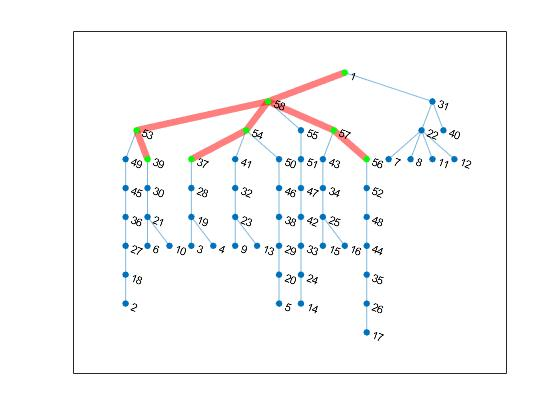
\includegraphics[width=1.0\linewidth]{f_c_map2.jpg}
  \caption{The tree structure of $M_0$}
\end{subfigure}
\begin{subfigure}{.45\textwidth}
  \centering
  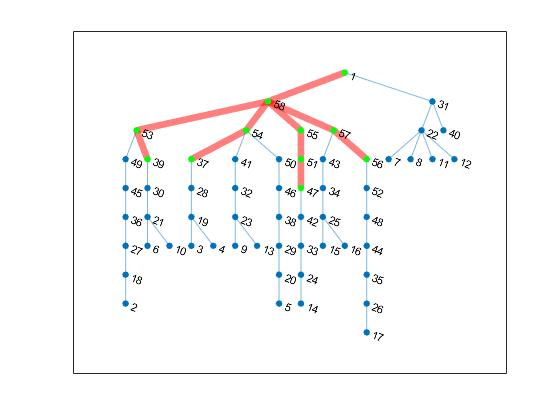
\includegraphics[width=1.0\linewidth]{alpha_0.jpg}
  \caption{The tree structure of $M_1$}
\end{subfigure}
\begin{subfigure}{.45\textwidth}
  \centering
  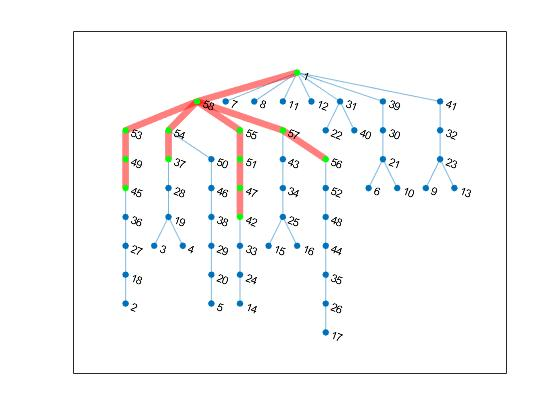
\includegraphics[width=1.0\linewidth]{alpha_1.jpg}
  \caption{The tree structure of $M_2$}
\end{subfigure}
\caption{The blue circles represent the ground set, the green circle represent the picked subgoals, and the red lines represent the path, respectively. There are six tree structures in map 2.}
\end{center}
\end{figure}

\begin{figure}[htbp]
\ContinuedFloat
\begin{center}
\begin{subfigure}{.45\textwidth}
  \centering
  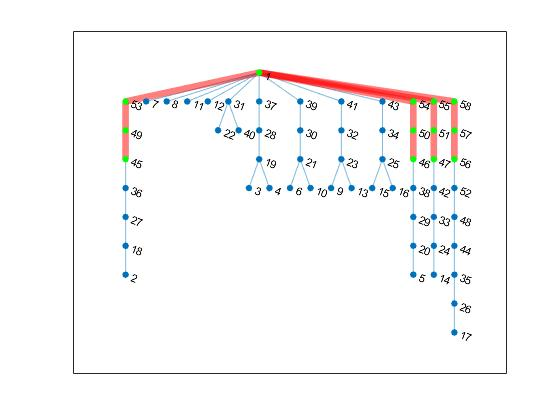
\includegraphics[width=1.0\linewidth]{alpha_2.jpg}
  \caption{The tree structure of $M_3$}
\end{subfigure}
\begin{subfigure}{.45\textwidth}
  \centering
  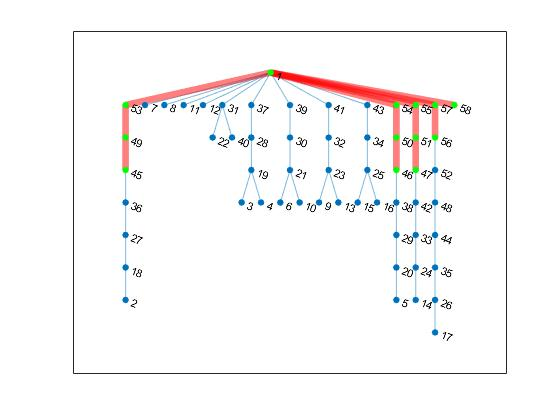
\includegraphics[width=1.0\linewidth]{alpha_3.jpg}
  \caption{The tree structure of $M_4$}
\end{subfigure}
\begin{subfigure}{.45\textwidth}
  \centering
  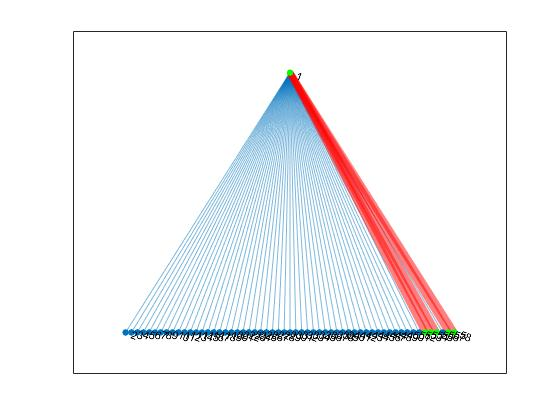
\includegraphics[width=1.0\linewidth]{alpha_4.jpg}
  \caption{The tree structure of $M_5$}
\end{subfigure}
\caption{The blue circles represent the ground set, the green circle represent the picked subgoals, and the red lines represent the path, respectively. There are six tree structures in map 2.}
\label{fig:trees_map2}
 \end{center}
 \end{figure} 